% !TEX root = ../notes.tex

\noindent\marginnote{\emph{Lecture 8}}[0mm]
We will let $u = \frac{N}{K}$, $v = \frac{P}{hk}$ and $\t = rt$. Then we substitute in,
\begin{align*}
  \di u \t &= \di N t \di u N \di t \t\\
  &= u - u^2 - \frac{uKk uhK}{K^2ru + KrD}\\
  &= u - u^2 - \frac{hK}{r}\frac{uv}{u + \frac{D}{k}}\\
  &= u - u^2 - \frac{auv}{u + d}
\end{align*}
that's the first equation dealt with, so we consider the other.
\begin{align*}
  \di v \t &= \di v P \di P t \di t \t \\
  &= \frac{1}{hKr} \left[ sP - \frac{sP}{hN} \right]\\
  &= \frac{s}{r}v \left(1 - \frac{v}{u}\right)\\
  &= bv\left( 1 - \frac{v}{u} \right)
\end{align*}

We are now going to consider the steady states of this system, we can't solve it as nicely using a graph. Our system is now going to live in $\R^2$. The part of the plane where both of them live is called the phase space. We will find trajectories that are tangents to these vector fields.\\

\subsection{Steady States}
The definition is still the same,
\begin{ndefi}[Steady State]
  A point $\vec u^*$ is a steady state if $\vec F(\vec u^*) = \vec 0$.
\end{ndefi}
What if only one component is zero? These are called the nullclines.
\begin{ndefi}[Nullclines]
  The $u_n$ nucline contains points $(u_1,\,u_2)$ such that $f_n(u_1, \, u_2) = 0$.
\end{ndefi}

Let's consider our system, we have,
\begin{align*}
  f_1(u,\,v) &= u(1- u) - \frac{auv}{u + d}\\
  f_2(u,\,v) &= bv \left(1 - \frac{v}{u}\right)\\
\end{align*}
and we find the nuclines are,
\begin{align*}
  v &= \frac{u(1 - u)(u + d)}{au} = 0\\
  u &= v \qquad \text{ or} v = 0
\end{align*}

\begin{figure}[!ht]
\centering
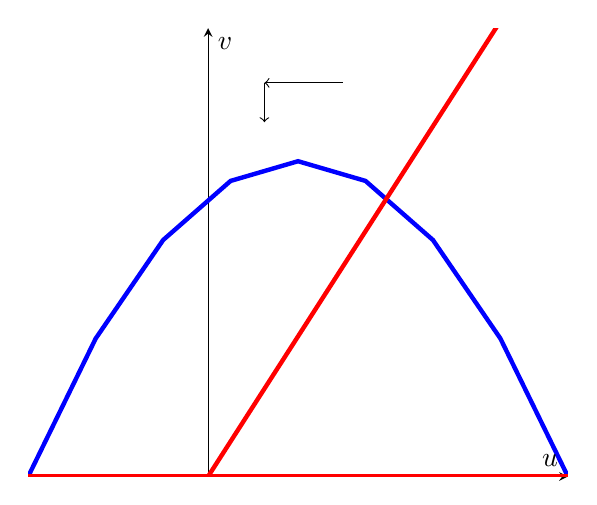
\begin{tikzpicture}[scale=1.0]
\begin{axis}[
        ticks = none,
        axis x line=middle,
        axis y line=middle,
        ymax=0.8, ymin=0, ylabel=$v$,
        xlabel=$u$
        ]
    \addplot[domain=-0.5:4, blue, ultra thick] {(1 - x) *(x + 0.5)};
    \addplot[domain=-0.5:3, red, ultra thick] {x};
    \addplot[domain=-0.5:1, red, ultra thick] {0};
\end{axis}
\draw[<-] (3,5) -- (4,5);
\draw[->] (3,5) -- (3,4.5);
\end{tikzpicture}
\caption{}
\end{figure}
We can now find the direction of the vector field using some quick calculation
